\section{Aufbau}
\label{sec:Aufbau}

\begin{figure}
\centering
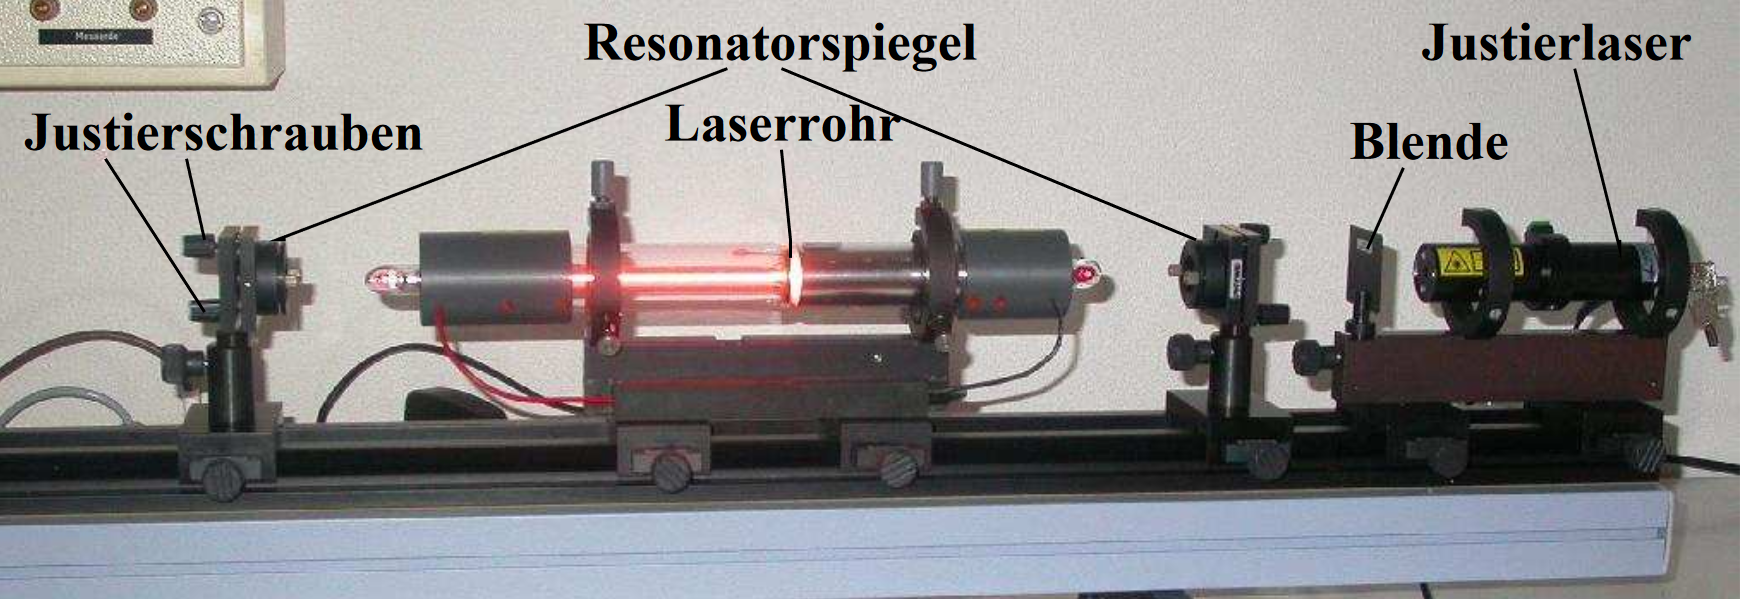
\includegraphics[width=0.8\textwidth]{content/images/aufbau.png}
\caption{Aufbau eines HeNe-Lasers auf einer optischen Schiene.\cite{V64}}
\label{fig:aufbau}
\end{figure}

\noindent Der Versuchsaufbau zur Untersuchung des HeNe-Lasers ist in Abbildung \ref{fig:aufbau} zu sehen.
Ein Laserrohr mit Helium-Neon-Gemisch, welches an beiden Enden mit Brewsterfenstern abgeschlossen und an eine Hochspannungsquelle angeschlossen ist, wird auf einer optischen Schiene montiert an deren einem Ende ein Justierlaser aufgebaut ist.
Desweiteren stehen verschiedene flache und gekrümmte Spiegel zur Verfügung um einen optischen Resonator zu bilden. Zur Untersuchung der Lasereigenschaften können außerdem ein Gitter, ein Polarisationsfilter, ein Draht und eine Photodiode montiert werden. 